\chapter{Targeted Firmware Rehosting}
\label{chap:rehost}

\begin{figure}
\centering
\begin{tikzpicture}[
  node distance=2cm,
  fuzzer/.style={rectangle, draw, text centered, rounded corners},
  container/.style={rectangle, draw, text centered},
  snapshot/.style={rectangle, draw, text centered, dashed},
  arrow/.style={->, >=stealth', shorten >=1pt, shorten <=1pt}
]

% Containers
\node (root) [container] {RAM File-system};

% CRIU snapshots
\node (snapshot1) [snapshot, left of=root, xshift=-2cm] {CRIU Snapshot};

\node (container1) [container, below left of=root] {Container 1};
\node (container2) [container, below right of=root] {Container $n$};

% Fuzzers
\node (fuzzer1) [fuzzer, below of=container1] {Fuzzer 1};
\node (fuzzer2) [fuzzer, below of=container2] {Fuzzer $n$};


% Arrows
\draw [arrow, very thick] (root) -- (container1);
\draw [arrow, very thick] (root) -- (container2);
\draw [arrow, very thick] (container1) -- (fuzzer1);
\draw [arrow, very thick] (container2) -- (fuzzer2);
\draw [arrow, very thick] (snapshot1) -- (root);
\end{tikzpicture}
\caption{The CRIU and Docker-based QEMU fuzzing system used to evaluate Jetset's rehosting of emulated systems.}
\label{fig:fuzzing}
\end{figure}

Embedded systems pose a challenge for emulation because their code expects to interact with specialized on-chip and off-chip peripherals, such as general-purpose I/O (GPIO) ports, sensors, and communication interfaces. 
In this dissertation, we consider this specific challenge in the context of \emph{rehosted} emulation.
Introduced in Chapter~\ref{chap:emulation}, rehosting refers to the decoding of information from a system specification into a set of emulated systems capable of executing that system in a different domain, e.g. a laptop computer.
The execution environment must emulate these devices with sufficient fidelity to ensure that observed behavior accurately mimics the target system running on hardware. 
However, because of the large variety of peripheral devices, most are not modeled by the execution environment, creating a considerable blind spot for our most powerful analysis techniques. 
Indeed, there may be no documentation at all about a target system, which makes building a complete emulator for it nearly impossible.

In many cases, however, the code of interest to the system analyst is not the code that interacts with peripherals. 
While peripherals cannot be ignored completely---hardware initialization must appear successful for the system to boot successfully---correct behavior of all devices may not be necessary. 
This chapter will focus on the rehosting approach, which attempts to infer partial but effective models of these missing hardware devices, and Chapter~\ref{chap:integreat} will look at an extraction based approach to this same problem.
For example, an analyst interested in how a target responds to network traffic may not require the execution environment to faithfully model all aspects of the system's GPIO ports or other communication interfaces.

The subject of this chapter is Jetset, a system that performs \textit{targeted rehosting} of firmware\textemdash it automatically infers the expected behavior of embedded system peripherals using only its firmware and then synthesizes a model of the peripherals sufficient to boot to security-critical code of interest. 
The synthesized peripheral model can then be used in an emulator---in our evaluation we used QEMU~\cite{bellard2005qemu}---to emulate the hardware environment. 
An analyst can then use her tool of choice to interact with the firmware. 
For example, a vulnerability analyst can use Jetset to fuzz-test the system to see how it responds to malformed or otherwise malicious input. 
More advanced dynamic analyses, like symbolic execution, are also available to the analyst.

Jetset infers the values that need to be read from peripheral devices needed for the program to reach an analyst-specified \emph{goal address}. 
For example, on the Raspberry Pi target used in our evaluation, our goal is to reach the address where the code jumps to user space. 
Our key insight is that firmware code interacting with a peripheral device implicitly encodes how the device must behave for the system to boot. 
Jetset uses symbolic execution of the firmware---specifically the angr framework~\cite{wang2017angr}---to infer data returned from devices.  

The input to Jetset is the executable firmware image, the firmware entry point (where to start execution), a goal address (the address we want to reach in execution), and a memory layout specifying which parts of the address space represent RAM and which represent memory-mapped I/O. 
Jetset only requires emulation support for the CPU architecture; it does not require any special hardware, and does not use the underlying hardware device.

To evaluate Jetset, we use it to infer and instantiate peripheral devices for thirteen targets: an aircraft Communication Management Unit (AMD 486-based system) used on the Boeing 737, Linux on a Raspberry Pi 2 (ARM-based SoC board), the first-stage bootloader on a BeagleBoard-xM (ARM-based SoC board), a SEL-751 Feeder Protection Relay (Motorola ColdFire-based system), and the 9 publicly available real-world targets from prior comparable work\cite{p2im2020}. 
These targets are diverse\textemdash they come from 3 different architectures, 5 different operating systems (as well as 3 different bare metal systems), and several different application domains.
For each target, Jetset inferred the behavior of its peripherals needed for the firmware to complete its boot sequence,and produced C code suitable for use with QEMU that simulates the inferred devices. 
We then run the firmware in QEMU configured for the target CPU architecture using our synthetic peripherals to complete the configuration.

For two of our targets, we confirm that the synthesized devices work
correctly by comparing the emulated system against a reference.  For
the Raspberry Pi 2, we compare the emulated behavior of the system to its
behavior on actual hardware.  
We used a novel framework capable of snapshotting the QEMU device emulator and instrumenting this with the AFL
fuzzer~\cite{zalewski2017technical} to fuzz-test the Linux
kernel system call interface, obtaining the same results both in QEMU
and on the actual hardware.  For the Communication Management Unit
(CMU), we use a high-fidelity QEMU implementation of the system,
including its most important peripherals for comparison.  We produced
this implementation by manually reverse-engineering the CMU as our
reference. We used our fuzzer to test the system call interface of the
underlying OS on both the reference and synthesized implementations to
confirm we observe the same behavior on both.  Although finding
vulnerabilities was not the goal of this testing, we nevertheless
identified a previously unknown privilege escalation vulnerability in
the VRTX kernel used by the CMU
(Section~\ref{sec:cmu-attack}).
This chapter will also discuss other exploits developed using this emulator analysis and disclosed to UTC aerospace: first, a local code execution method based upon the data loader protocol, and ACARS messages which are capable of disabling a running CMU remotely.

\section{Related Work on Rehosting}
\label{sec:rehost-related}

Due to the complex nature of firmware and the heterogeneity of the hardware it interacts with, security testing and analysis of firmware is a difficult problem~\cite{muench2018you, wright2021challenges}.
Different techniques to test and analyze firmware vary both in their goal (e.g., finding bugs, full rehosting, or partial rehosting), as well as the assumptions that they make about the firmware they analyze.
For example, a testing technique may only analyze firmware using a particular operating system~\cite{firmadyne}, or may assume that auxiliary information about the firmware is available (e.g., firmware-hardware I/O traces~\cite{pretender2019}) to improve results.
The use case of Jetset\textemdash partial rehosting using only the firmware itself and no auxiliary information\textemdash is most similar to other rehosting techniques, however, for completeness, we outline other approaches to analyzing firmware below.

\paragraph{Firmware testing and analysis}
Approaches have been developed to test firmware without attempting to create a stand-alone emulator for the hardware.

Symdrive~\cite{symdrive} is a symbolic testing framework for Linux device drivers.
Symdrive takes as input the C code for the Linux drivers and attempts to find program paths that violate user written assertions. 
Symdrive is able to uncover numerous bugs in Linux device drivers; however, it requires source code and is Linux specific.

FIE~\cite{fie} is a symbolic execution framework that targets firmware for the
MSP430 family of microprocessors.
FIE takes as input a piece of firmware, a memory map (that denotes which regions are RAM, ROM, MMIO, etc), and an interrupt specification which describes all locations where interrupts could be fired. 
FIE is designed to analyze all firmware execution paths, which, while effective for the simpler MSP430 microcontroller firmware, is not feasible for more complex firmware like the Raspberry Pi's Linux kernel. 
For this complex firmware, a more targeted approach such as Jetset's is needed.
Furthermore, FIE requires the source code for the firmware\textemdash this is how it adds its symbolic execution instrumentation\textemdash and it is therefore unsuitable for our needs.

Revnic~\cite{revnic} is a system for symbolically executing driver firmware and reverse engineering its functionality.
Revnic takes as input a driver binary, a driver template describing the high level functionality of the driver, and domain specific knowledge about the OS of the driver, and produces source code for the driver.
Revnic requires knowledge of the underlying operating system, and requires that the user provide detailed device templates that outline the functionality of the device, and it is therefore unsuitable for the problem of firmware-only emulation.

FirmUSB~\cite{firmusb} is a USB-specific symbolic execution framework for analyzing USB microcontroller firmware. 
FirmUSB takes as input a USB firmware image, and uses domain specific analyses  to identify malicious behavior by the USB device.
For example, FirmUSB can detect if a device claiming to be a USB keyboard is injecting keys that have not been pressed by looking for USB specific information flows.

\paragraph{Hardware-in-the-loop emulation} 
Another method of approaching the problem of analyzing firmware is to attach a software emulator running the firmware to the physical hardware, forwarding I/O between the emulator and the firmware.
Avatar~\cite{avatar} is a dynamic analysis framework for embedded systems that does exactly this.
Other tools 
\textsc{Surrogates}~\cite{surrogates} and \textsc{Prospect}~\cite{kammerstetter2014prospect} build on this hardware-in-the-loop approach.

This technique provides the highest fidelity emulation since the emulator directly interacts with the physical hardware; however, use of this technique is contingent on continuous access to the hardware, which is not always possible since hardware (like that used in avionics) may be difficult or impossible to obtain.

\paragraph{Full firmware rehosting} 
Full rehosting is a technique which attempts to construct a fully featured, high-fidelity emulator from a piece of firmware and auxiliary information about the SoC or firmware.

Firmadyne~\cite{firmadyne} is a platform for automated dynamic analysis of Linux-based embedded systems.
Firmadyne takes as input a piece of firmware running the Linux kernel, and executes user-space code for the firmware, emulating the common Linux peripherals.
Similarly, Costin et al.~\cite{costin2014large, costin2016automated} extract and rehost the embedded system's filesystem in their own analysis environment to analyze network-facing code.
Because the code of interest to an embedded system security analyst is often the user-space, network-facing code, Firmadyne and Costin et al.'s tool are well-suited for this scenario. 

Pretender~\cite{pretender2019} rehosts firmware by recording the interactions between the physical hardware and the firmware. 
It then uses a machine learning engine to learn a stateful model for peripheral behavior and creates an emulator from this model.
Similar to Avatar, Pretender takes as input the firmware, and a connection to the physical hardware, and creates an emulation environment; however, unlike Avatar and related tools, Pretender can fully migrate the firmware to a virtualized environment, and does not require persistent access to the hardware.


HALucinator~\cite{clementshalucinator} is a firmware rehosting tool that uses hueristics to locate the code belonging to the hardware abstraction layer (a vendor-provided API for interacting with the hardware) in the firmware and replaces it with manually created handlers. 
HALucinator takes as input firmware, and the HAL the firmware uses, and produces a fully featured emulation environment for the firmware.


Previous rehosting techniques have relied on auxiliary information to infer the behavior of the hardware environment.
While this results in a more complete emulator, this auxiliary information is not always available\textemdash most of our evaluation subjects had none.
Furthermore, security analysis is often concerned with only a particular software component of the firmware, (e.g., the network traffic or the file system code) and may not need a fully featured emulator.

\paragraph{Partial rehosting}
Partial rehosting, as opposed to full rehosting, attempts to create an emulator from the firmware only, with no auxiliary information about the peripherals.
However, the emulators produced by partial rehosting are not complete\textemdash they are not guaranteed to implement all peripherals for the firmware, only what they can infer.
This is the point in the design space that Jetset occupies.
There is one other notable system that implements partial rehosting, P\textsuperscript{2}IM.

P\textsuperscript{2}IM~\cite{p2im2020} does both fuzzing and partial rehosting based on the peripheral model that it infers from the fuzzing stage.
It takes as input the target firmware and its memory map, and fuzzes the firmware code by channeling input from an off-the-shelf fuzzer like AFL to the peripherals. 
It then analyzes the device access patterns exercised during this fuzzing pass to infer details about the memory-mapped IO interactions between the firmware and peripheral devices, and executes the firmware without crashing.

There are two key differences between P\textsuperscript{2}IM's fuzzing-based approach, and Jetset's directed symbolic execution-based approach.
The first difference is that unlike P\textsuperscript{2}IM, Jetset is \textit{targeted}\textemdash it is designed to ignore most paths through the firmware to focus on a particular target piece of code, which allows it boot deep into large pieces of firmware.
While Feng et al. showed P\textsuperscript{2}IM's approach is effective at fuzzing peripheral handling code and emulating microcontroller code, it is not clear whether it scales to larger firmware.
Besides evaluating against all of P\textsuperscript{2}IM's publicly available real-world evaluation subjects, we also evaluated Jetset against four complex pieces of firmware\textemdash one of our evaluation subjects, the Raspberry Pi 2 is 450x LoC of any of P\textsuperscript{2}IM's evaluation subjects.
We attempted to evaluate P\textsuperscript{2}IM on our 4 real-world firmware samples. Unfortunately, the current version of P\textsuperscript{2}IM only supports Cortex-M MCUs and we were unable to run it on any of our samples, including our Cortex-A7 and Cortex-A8 firmware.

The second difference is that, while fuzzing-based approaches are efficient since they use lightweight executions, they can have trouble bypassing complex checks. 
In Section~\ref{sec:jetset-eval}, we provide an example of a complex numerical check that occurred when inferring the behavior of an FPGA in one of our evaluation subjects.
Jetset is able to handle complex numerical checks, because it performs partial rehosting using symbolic execution.

\section{Jetset's Inference of Hardware Semantics}
\label{sec:jetset-eval}

Jetset uses symbolic execution to infer how peripheral devices must respond to reads from the firmware for execution to progress toward the goal address.
It uses this inferred information to deduce and reproduce expected peripheral device functionality to boot firmware in an emulator such as QEMU.
This allows analysts to boot the system in an emulator with only the firmware, and without the target's hardware or support for the peripheral devices in the emulator.
To do this, Jetset requires the following information about the target embedded system (discussed briefly in Chapter~\ref{chap:emulation}).

\begin{itemize}[noitemsep, leftmargin=12pt]
\item The \emph{executable code} of the target, usually read out of program flash or extracted from a firmware update provided by a manufacturer.
\item The \emph{memory layout} of the target, specifying which regions of the address space are mapped to program memory, RAM, and device I/O registers.
This information can be obtained from the data-sheet of a single-chip system or from a basic analysis of the executable code. Note that Jetset does \emph{not} need to know which devices are mapped where, only the address range used for memory-mapped I/O.
\item The \emph{entry point address} where execution begins.
This is often specified in the CPU data-sheet.
\item The program \emph{goal address} that the analyst wants the program to reach.
For example, this can be the address of a print instruction that reports a successful system boot.
\end{itemize}

To model peripherals, Jetset uses symbolic execution to \emph{infer} expected device behavior, and then the resulting encoding of the device behavior in the constraints returned by symbolic execution is used to \emph{synthesize} a device suitable for use in an emulator (e.g., QEMU).
Secondary to this \emph{peripheral Modeling} phase, Jetset must also adopt a correct \emph{search strategy} to guide symbolic execution, introduced in Chapter~\ref{chap:prelim}.

\subsection{Jetset's Peripheral Modeling}
In its \emph{peripheral inference} stage, Jetset symbolically executes the firmware to infer what values should be returned by reads from device registers in order for execution to reach the firmware's goal address.
In Jetset, input from devices are marked symbolic and tracked through QEMU's emulation by \emph{taint-tracking} all Tiny Code Generator (TCG) operations and a number of QEMU's helper functions.
During execution, all reads from memory-mapped I/O addresses space are therefore symbolic, while the initial contents of flash and memory are concrete.\footnote{Note that this means Jetset \emph{does not} infer flash devices, something which was manually modeled for the emulation during the QEMU exploit generation.}
Each read from a memory-mapped I/O address returns a distinct symbolic variable; that is, two reads from the same address result in two \emph{different} symbolic values.
Jetset stops when an execution path reaches the goal address, resulting in a set of constraints on values read from device registers that lead to this address.

\paragraph{Interrupts}
While executing, the firmware may also require interrupts to be serviced to reach the target.
Jetset therefore periodically injects interrupts during the modeling stage.
For example, the goal address for the Raspberry Pi firmware is in a different kernel thread than the entry point, so a scheduler interrupt is needed to reach the goal.
From Jetset's point of view, this means that it needs to execute an interrupt service routine (ISR) to make progress.
Given infinite compute resources, Jetset could explore every possible interrupt either firing or not after each instruction.
However, this is impractical.
Jetset exploits the fact that well-designed systems are not sensitive to the \emph{exact} timing of interrupts and that ISRs are written to handle spurious interrupts gracefully.
Jetset periodically injects interrupts during symbolic execution, so that each ISR is executed periodically during each execution path.
If the main execution thread happens to be waiting for an ISR to update a variable, Jetset will eventually execute that ISR, and the thread can continue making progress.

\paragraph{Peripheral synthesis}
Once Jetset has reached the target (with or without interrupts), it can create a synthetic peripheral model that can be used in QEMU.
The result of the inference stage is a set of constraints on values read from peripherals needed for the firmware to boot.
Jetset then uses Z3~\cite{zthree}, the default SMT solver used by angr, to find concrete values satisfying these constraints, capturing in the firmware's expected response to device reads during execution.
This allows Jetset to construct a light-weight, concrete device model, rendering peripheral modeling a one-time cost per device.

This synthesis stage generates an I/O trace model that is sufficient to reach the goal in the emulator.
The synthesized trace is partitioned by I/O address, so there is a separate trace for each memory-mapped I/O address.
When Jetset reaches the end of an I/O trace for a particular address, any subsequent reads return the last value in the trace.
This allows Jetset to continue past the goal address in emulation, but precludes any complex interaction with the device after the trace has ended (see Section~\ref{sec:jetset-limitations}).

The synthesized device injects interrupts in the same way as during peripheral modeling, ensuring that any necessary ISRs are executed in emulation.
Interrupt timing during execution in an emulator does not need to precisely match the timing during peripheral modeling\textemdash if, during emulation, an interrupt is fired one instruction later, this will not make a difference in emulation.

\subsection{Jetset's Search Strategy}

To ensure that Jetset continues to make forward progress towards the goal address during symbolic execution, which by default attempts to explore the all executable paths, Jetset uses a distance function to guide its search.
This distance function is context-sensitive~\cite{directedsymex}: it takes into account that the distance between two instructions in a program can depend on the calling contexts (i.e., the callstack) of the two instructions.
Computing a context-sensitive distance function is more complicated than computing a local distance (i.e., the distance between two instructions in a single function).
Whenever a decision point is encountered, Jetset chooses the shortest path to the goal location, barring a few exceptions, discussed later.

\begin{figure}
\centering
% Adapted from http://www.texample.net/tikz/examples/flexible-flow-chart/
\newcounter{step}
\newcommand*\step{
  \stepcounter{step}%
  \scriptsize
  \arabic{step}.
  \ttfamily
}
\begin{tikzpicture}[
  % Global options.
  >=Stealth,
  node distance=2.5ex,
  every join/.style={norm},
  every label/.style={font=\scriptsize},
  % Flow chart box styles.
  base/.style={font=\step, draw, on chain, on grid, align=center, minimum height=2ex, inner xsep=.1em, top color=black!10},
  proc/.style={base, rectangle, minimum width=4em},
  test/.style={base, diamond, aspect=2, minimum width=4em},
  % Connector styles.
  norm/.style={shorten >=1pt, ->, font=\scriptsize, pos=.3333},
  % Outline styles.
  outline/.style={draw, rectangle, densely dotted, rounded corners, inner sep=1ex},
]
% CFG for main.
{[start chain=main going below]
  \node[proc]                {call foo};
  \node[proc, join=by {"2"}] {call bar};
  \node[proc, join=by {"3"}] {call foo};
  \node[proc, join=by {"2"}] {ret};
}
\node[outline, fit=(main-begin) (main-end), label={\texttt{main} ($\mathit{length}=7$)}] {};

% CFG for foo.
{[start chain=foo going below]
  \node[proc, right=3 of main-begin] {mem[0x100] = 1};
  \node[proc, join=by {"1"}]       {eax = 2};
  \node[proc, join=by {"1"}]       {ret};
}
\node[outline, fit=(foo-begin) (foo-end), label={\texttt{foo} ($\mathit{length}=2$)}] {};

% CFG for bar.
{[start chain=bar going below]
  \node[proc, right=3.5 of foo-begin] {ebx = mem[0x200]};
  \node[test, join=by {"1"}]      {ebx == 1};
  {[start branch=then]}
  \node[proc, join=by {"\texttt{false}; 1"}] (cond) {eax = 3};
  {[continue branch=then]
    \node[proc, right=1.75 of cond,
          join=by {rounded corners,
                   to path={-|(\tikztotarget) \tikztonodes},
                   pos=.25,
                   "\texttt{true}; 1"}] {eax = 2};
  }
  \node[on chain] (dummy) {};
  \node[proc,
        join=with cond by {"1"},
        join=with bar/then-end by {
          -,
          rounded corners,
          to path={|- (dummy) \tikztonodes -| (\tikztotarget)},
          "1"}] {ret};
}
\node[outline, fit=(bar-begin) (bar/then-end) (bar-end), label={\texttt{bar} ($\mathit{length}=3$)}] {};
\end{tikzpicture}

% vim: set sw=2 sts=2 ts=8 et tw=0:

\caption{Context-sensitive distance from statement 5 (in first \texttt{foo} call) to statement 7 (of second \texttt{foo} call).}
\label{fig:jetset-distance-func}
\end{figure}

The local distance between two instructions is simply the graph distance between the two instructions in the control flow graph.
For example, in Figure~\ref{fig:jetset-distance-func}, the distance from statement 5 to statement 7 (both within \texttt{foo}) is 2.
When computing local distances, the edges for call instructions need to be weighted based on the called function's \textit{length}\textemdash the distance between the start of the called function and the nearest return of that function.
For example, in Figure~\ref{fig:jetset-distance-func}, the distance from statement 1 to statement 4 is not 3, but 7.
This is because, when executing a call instruction, it is not really one instruction being executed, but every instruction until the call returns.
This is further complicated, because the called function may itself call other functions.
Therefore, to compute local distances for each function, Jetset first creates a callgraph of all functions in the firmware, then computes local distances for functions in topographical order.
This ensures that when Jetset computes local distances for a function, it has already computed local distances for every function that function calls.
But this still only gives local distances\textemdash it does not provide distances between instructions in different functions.

Computing the distances between instructions in different functions is more complicated, because functions are often called in more than one context and Jetset is only interested in \textit{realizable paths}\textemdash paths which follow a valid call-return sequence.
For example, in Figure~\ref{fig:jetset-distance-func}, the distance between statement 5 (in \texttt{foo}) and statement 4 (in \texttt{main}) depends on \texttt{foo}'s calling context: if \texttt{foo} was called from statement 1, then the distance is 7, if \texttt{foo} was called from statement 3, then the distance is 2.

Jetset uses a context-sensitive distance function: it determines the distance between an instruction in one calling context\textemdash a (pc, callstack) pair\textemdash to another instruction, in another calling context.
To compute this distance function, Jetset first precomputes local distances for all functions.
Then, Jetset computes the distances between instructions in different functions.
To do this, Jetset takes advantage of the fact that all paths between instructions can be broken up into a sequence of returns, followed by a sequence of calls~\cite{directedsymex} (there will never be an interleaved call and return, because then that would be a local distance!).
Nonlocal distances can therefore be separated into two distances: the \textit{callstack distance}\textemdash the distance along the sequence of returns up the callstack\textemdash and the \textit{callchain distance}\textemdash the distance along the sequence of calls that lead to the goal address (or the goal address in a specific calling context).

Jetset precomputes all local distances, but both the callstack and callchain distances are computed lazily from the actual stack during execution (it is infeasible to precompute all callstack and callchain distances).
Jetset computes the total context-sensitive distance as the sum of the callstack and callchain distances.

The callstack distance measures the distance from an instruction in one calling context to an instruction that can be reached by a sequence of returns (i.e., instructions in functions in the current callstack).
To compute the callstack distance, Jetset first computes the local distance to the location of the closest \texttt{return} instruction.
It continues summing the distances to each return of each function recursively up the call stack.
It stops once it reaches a function that can reach the target with a set of calls (i.e., a function that is in the target's callstack):

\begin{lstlisting}[language=python]
# Calculate callstack distance
while function not in target_callstack:
  distance += local_distance(cur, ret)
  cur = function.returns_to
  function = stack.next_function  
\end{lstlisting}

For example, suppose Jetset wanted to reach statement 7 (in the second \texttt{foo} call) from statement 5 (in the first \texttt{foo} call).
The call stack distance would be 2, as that is the distance to exit from \texttt{foo} to \texttt{main}, at which point statement 7 can be reached by a set of calls.

The callchain distance measures the distance from an instruction in one calling context to an instruction that can be reached by a sequence of calls.
To compute the callchain distance, Jetset first computes the local distance to the nearest \texttt{call} instruction that leads to the target.
It then recursively sums the distance to each function call on the way to the target:

% break page
\newpage

\begin{lstlisting}[language=python]
# Calculate callchain distance
while function != target_function:
  call = target_callstack.closest_call
  distance += local_distance(cur, call)
  function = call.target
  cur = function.entry     
\end{lstlisting}

Suppose again  that Jetset wanted to reach statement 7 (in the second \texttt{foo} call) from statement 5 (in the first \texttt{foo} call).
The call chain distance would be 5: 3 to reach the second \texttt{foo} call and 2 to descend into the \texttt{foo} call to reach statement 7.

\paragraph{Search Exceptions}
However, there are many cases where due to incomplete semantic modeling and software control flow complexity, Jetset is not able to identify a correct path to the current goal address using the context-sensitive CFG.
For example, to cope with loops where taking the shortest path will lead to a hanging state, we \emph{alternate} decisions, to avoid taking the same branch twice where unnecessary.
For these cases, Jetset relies on using the local distance to the nearest return as a fallback distance function.
The incremental CFG generation improves the quality of the CFG over time, so eventually the CFG will contain a path to the target.

Jetset's search algorithm may also guide it to a point in the program where it becomes infeasible to reach the target and it needs to terminate the current path and backtrack to a previous state.
There are two different cases where this occurs.
The first case where Jetset backtracks is when a system reset occurs; it is unlikely that a system reset takes place in a correct boot sequence, and backtracking on system resets allows Jetset to avoid boot loops.
The second case where Jetset backtracks is when Jetset enters a statically-detectable infinite loop.
It is also possible to set explicit ``avoid'' locations which will force Jetset to backtrack if some set of constraints are satisfied.

\section{Evaluating Jetset's Targeted Rehosting}

% Targets Data
\newcommand\mmio{MMIO\xspace}
\newcommand\rpitwo{Raspberry Pi 2\xspace}
\newcommand\cmutarg{CMU-900\xspace}
\newcommand\seltarg{SEL-751\xspace}

\newcommand\comma[1]{\num[group-separator={,}]{#1}}

\newcommand\rpiInfWallClockTime{6m43s}
\newcommand\rpiInfBlocksInCode{238,792}
\newcommand\rpiInfRawTotalBlocks{81194393}
\newcommand\rpiInfTotalBlocks{\num[group-separator={,}]{\rpiInfRawTotalBlocks}}
\newcommand\rpiInfTotalBlocksOnPath{81,194,393}
\newcommand\rpiInfUniqueBlocks{43,157}
\newcommand\rpiInfUniqueBlocksOnPath{43,157}
\newcommand\rpiInfWritesOnPath{84,060}
\newcommand\rpiInfReadsOnPath{83,857}
\newcommand\rpiInfWriteAddressesOnPath{40}
\newcommand\rpiInfReadAddressesOnPath{37}
\newcommand\rpiInfDevicesAccessed{6}


\newcommand\rpiSynthWallClockTime{3.16s}
\newcommand\rpiSynthSymbolicVars{1,384}
\newcommand\rpiSynthTotalConstraints{5,226}
\newcommand\rpiSynthAvgConstraints{3.78}
\newcommand\rpiSynthMedConstraints{4}
\newcommand\rpiSynthMaxConstraints{30}
\newcommand\rpiSynthAvgTraceLen{37.4}
\newcommand\rpiSynthMedTraceLen{1}
\newcommand\rpiSynthMaxTraceLen{1076}


\newcommand\rpiEmuWallClockTime{8s}

\newcommand\rpiEmuRawTotalBlocks{81454594}
\newcommand\printpercent[2]{\FPeval\result{round(#1*100/#2,1)}\result\%}
\newcommand\printpercentmore[2]{\FPeval\result{round(#1/#2-1,1)}\result\%}
\newcommand\rpiRawEmuTotalBlocks{43227}
\newcommand\rpiEmuTotalBlocks{\num[group-separator={,}]{\rpiEmuRawTotalBlocks}}
\newcommand\rpiEmuPercBlocksMore{\printpercentmore{\rpiEmuRawTotalBlocks}{\rpiInfRawTotalBlocks}}

\newcommand\rpiEmuUniqueBlocks{43,255}
\newcommand\rpiEmuWritesOnPath{83,915}
\newcommand\rpiEmuReadsFromTrace{83,857}
\newcommand\rpiEmuReadsBeyondTrace{0}
\newcommand\rpiEmuWriteAddresses{43}
\newcommand\rpiEmuReadAddresses{27}
\newcommand\rpiEmuDevicesAccessed{6}
                                                                           
\newcommand\bbxmInfWallClockTime{5m15s}
\newcommand\bbxmInfBlocksInCode{872}
\newcommand\bbxmInfTotalBlocks{20,198,824}
\newcommand\bbxmInfTotalBlocksOnPath{20,198,824}
\newcommand\bbxmInfUniqueBlocks{484}
\newcommand\bbxmInfUniqueBlocksOnPath{484}
\newcommand\bbxmInfWritesOnPath{938}
\newcommand\bbxmInfReadsOnPath{3,633}
\newcommand\bbxmInfWriteAddressesOnPath{244}
\newcommand\bbxmInfReadAddressesOnPath{61}
\newcommand\bbxmInfDevicesAccessed{11}


\newcommand\bbxmSynthWallClockTime{5.64s}
\newcommand\bbxmSynthSymbolicVars{\bbxmInfReadsOnPath}
\newcommand\bbxmSynthTotalConstraints{8,353}
\newcommand\bbxmSynthAvgConstraints{2.30}
\newcommand\bbxmSynthMedConstraints{2}
\newcommand\bbxmSynthMaxConstraints{74}
\newcommand\bbxmSynthAvgTraceLen{59.56}
\newcommand\bbxmSynthMedTraceLen{3}
\newcommand\bbxmSynthMaxTraceLen{2,770}

\newcommand\bbxmEmuWallClockTime{101ms}
\newcommand\bbxmEmuTotalBlocks{20,198,656}
\newcommand\bbxmEmuUniqueBlocks{483}
\newcommand\bbxmEmuWritesOnPath{938}
\newcommand\bbxmEmuReadsFromTrace{3,633}
\newcommand\bbxmEmuReadsBeyondTrace{0}
\newcommand\bbxmEmuWriteAddresses{244}
\newcommand\bbxmEmuReadAddresses{61}
\newcommand\bbxmEmuDevicesAccessed{11}
                                                                           
\newcommand\cmuInfWallClockTime{5m20s}
\newcommand\cmuInfBlocksInCode{55,016}
\newcommand\cmuInfTotalBlocks{53,143,508}
\newcommand\cmuInfRawTotalBlocksOnPath{27517932}
\newcommand\cmuInfTotalBlocksOnPath{\num[group-separator={,}]{\cmuInfRawTotalBlocksOnPath}}
\newcommand\cmuInfUniqueBlocks{776}
\newcommand\cmuInfUniqueBlocksOnPath{731}
\newcommand\cmuInfWritesOnPath{1,308}
\newcommand\cmuInfReadsOnPath{242}
\newcommand\cmuInfWriteAddressesOnPath{13}
\newcommand\cmuInfReadAddressesOnPath{5}
\newcommand\cmuInfDevicesAccessed{5}


\newcommand\cmuSynthWallClockTime{0.018s}
\newcommand\cmuSynthSymbolicVars{\cmuInfReadsOnPath}
\newcommand\cmuSynthTotalConstraints{756}
\newcommand\cmuSynthAvgConstraints{3.12}
\newcommand\cmuSynthMedConstraints{3}
\newcommand\cmuSynthMaxConstraints{11}
\newcommand\cmuSynthAvgTraceLen{48.4}
\newcommand\cmuSynthMedTraceLen{5}
\newcommand\cmuSynthMaxTraceLen{215}

\newcommand\cmuEmuWallClockTime{289ms}
\newcommand\cmuEmuRawTotalBlocks{27519080}
\newcommand\cmuEmuTotalBlocks{\num[group-separator={,}]{\cmuEmuRawTotalBlocks}}
\newcommand\cmuEmuUniqueBlocks{731}
\newcommand\cmuEmuWritesOnPath{1,882}
\newcommand\cmuEmuReadsFromTrace{242}
\newcommand\cmuEmuReadsBeyondTrace{0}
\newcommand\cmuEmuWriteAddresses{13}
\newcommand\cmuEmuReadAddresses{5}
\newcommand\cmuEmuDevicesAccessed{5}
                                                                           
\newcommand\selInfWallClockTime{2h34m51s}
\newcommand\selInfBlocksInCode{141,750}
\newcommand\selInfTotalBlocks{3,351,484,857}
\newcommand\selInfTotalBlocksOnPath{3,351,484,857}
\newcommand\selInfUniqueBlocks{11,364}
\newcommand\selInfUniqueBlocksOnPath{11,364}
\newcommand\selInfWritesOnPath{32,480}
\newcommand\selInfReadsOnPath{704}
\newcommand\selInfWriteAddressesOnPath{68}
\newcommand\selInfReadAddressesOnPath{26}
\newcommand\selInfDevicesAccessed{5}


\newcommand\selSynthWallClockTime{5.61s}
\newcommand\selSynthSymbolicVars{\selInfReadsOnPath}
\newcommand\selSynthTotalConstraints{11,142}
\newcommand\selSynthAvgConstraints{15.83}
\newcommand\selSynthMedConstraints{5}
\newcommand\selSynthMaxConstraints{1279}
\newcommand\selSynthAvgTraceLen{27.08}
\newcommand\selSynthMedTraceLen{2}
\newcommand\selSynthMaxTraceLen{343}

\newcommand\selEmuWallClockTime{1m1s}
\newcommand\selEmuTotalBlocks{3,351,502,947}
\newcommand\selEmuUniqueBlocks{11,364}
\newcommand\selEmuWritesOnPath{32,480}
\newcommand\selEmuReadsFromTrace{704}
\newcommand\selEmuReadsBeyondTrace{0}
\newcommand\selEmuWriteAddresses{68}
\newcommand\selEmuReadAddresses{26}
\newcommand\selEmuDevicesAccessed{5}

% Misc
\newcommand\numCmuVulns{1}
\newcommand\dtbFileDevices{28}
\newcommand\rpiDistinctSyscalls{1,571,576}

\newcommand\numXloadRegns{200}
\newcommand\numXloadSynDevs{TODO}
\newcommand\numHrsXload{TODO}
\newcommand\numLinxBrch{TODO}
\newcommand\numLinxIndrJumps{TODO}

% RPI Eval Data
\newcommand\rpiSyscallsIssued{}
\newcommand\rpiRawNumPathsDiscovered{123198}
\newcommand\rpiNumPathsDiscovered{\num[group-separator={,}]{\rpiRawNumPathsDiscovered}}
\newcommand\rpiHexDumpDiffsNum{51,592}
\newcommand\rpiHexDumpDiffsPerc{41.9\%}
\newcommand\rpiRawNumDeaths{51638}
\newcommand\rpiNumDeaths{\num[group-separator={,}]{\rpiRawNumDeaths}}
\newcommand\subtract[2]{\FPeval\result{round(#1-#2,0)}\comma{\result}}
\newcommand\rpiNumReturns{71560}
\newcommand\rpiPhysicalTestCases{14,661}

% CMU Eval Data
\newcommand\cmuRawNumPathsDiscovered{2963}
\newcommand\cmuNumPathsDiscovered{\comma{\cmuRawNumPathsDiscovered}}
\newcommand\cmuHoursFuzzed{200}
\newcommand\cmuRawExactOutputMatches{2884}
\newcommand\cmuExactOutputMatches{\comma{\cmuRawExactOutputMatches}}
\newcommand\cmuNearExactOutputMatches{36}
\newcommand\cmuNonExactOutputMatches{43}
\newcommand\cmuDifferenceInBlocksExecuted{\subtract{\cmuEmuRawTotalBlocks}{\cmuInfRawTotalBlocksOnPath}}

\newcommand\cmuPercentNonExactOutputToPaths{1.5\%}
\newcommand\cmuPercentNearOutputToPaths{1.2\%}
\newcommand\cmuPercentExactOutputToPaths{97.3\%}

\newcommand\bbxmDatasheetPeris{35}

\begin{table*}
\centering
\caption{Jetset's primary targets and summary statistics regarding peripheral modeling.}
\label{tab:targets}
\begin{tabular}{@{}lllrrrr@{}}
  \toprule
  \quad                       &                                                     & \multicolumn{2}{r}{\textbf{RPi2}} & \textbf{BBXM}      & \textbf{CMU-900}            & \textbf{SEL-751}            \\
  \midrule
  \multicolumn{2}{@{}l}{OS/SW}   & \multicolumn{2}{r}{Linux 4.19.y}                 & X-Loader                                   & VRTX-32                      & G5.1.5.0                                                  \\
  \multicolumn{3}{@{}l}{\emph{Peripheral inference}}                                                                                                                                                                        \\
                              & \multicolumn{2}{l}{Wall-clock time}                 & \rpiInfWallClockTime                        & \bbxmInfWallClockTime        & \cmuInfWallClockTime        & \selInfWallClockTime        \\
                              & \multicolumn{2}{l}{Blocks in code base}             & \rpiInfBlocksInCode                         & \bbxmInfBlocksInCode         & \cmuInfBlocksInCode         & \selInfBlocksInCode         \\
                              & \multicolumn{2}{l}{Total blocks executed}           & \rpiInfTotalBlocks                          & \bbxmInfTotalBlocks          & \cmuInfTotalBlocks          & \selInfTotalBlocks          \\
                              & \multicolumn{2}{l}{Blocks executed on path}         & \rpiInfTotalBlocksOnPath                    & \bbxmInfTotalBlocksOnPath    & \cmuInfTotalBlocksOnPath    & \selInfTotalBlocksOnPath    \\
                              & \multicolumn{2}{l}{Unique blocks executed}          & \rpiInfUniqueBlocks                         & \bbxmInfUniqueBlocks         & \cmuInfUniqueBlocks         & \selInfUniqueBlocks         \\
                              & \multicolumn{2}{l}{Unique blocks executed on path}  & \rpiInfUniqueBlocksOnPath                   & \bbxmInfUniqueBlocksOnPath   & \cmuInfUniqueBlocksOnPath   & \selInfUniqueBlocksOnPath   \\
                              & \multicolumn{2}{l}{\mmio\ writes (ignored) on path} & \rpiInfWritesOnPath                         & \bbxmInfWritesOnPath         & \cmuInfWritesOnPath         & \selInfWritesOnPath         \\
                              & \multicolumn{2}{l}{\mmio\ reads (symbolic) on path} & \rpiInfReadsOnPath                          & \bbxmInfReadsOnPath          & \cmuInfReadsOnPath          & \selInfReadsOnPath          \\
                              & \multicolumn{2}{l}{\mmio\ write addresses on path}  & \rpiInfWriteAddressesOnPath                 & \bbxmInfWriteAddressesOnPath & \cmuInfWriteAddressesOnPath & \selInfWriteAddressesOnPath \\
                              & \multicolumn{2}{l}{\mmio\ read addresses on path}   & \rpiInfReadAddressesOnPath                  & \bbxmInfReadAddressesOnPath  & \cmuInfReadAddressesOnPath  & \selInfReadAddressesOnPath  \\
                              & \multicolumn{2}{l}{Devices accessed}                & \rpiInfDevicesAccessed                      & \bbxmInfDevicesAccessed      & \cmuInfDevicesAccessed      & \selInfDevicesAccessed      \\
  % Fix to be just the peripherals
  \multicolumn{3}{@{}l}{\emph{Peripheral synthesis}}                                                                                                                                                                            \\
                              & \multicolumn{2}{l}{Wall-clock time}                 & \rpiSynthWallClockTime                      & \bbxmSynthWallClockTime      & \cmuSynthWallClockTime      & \selSynthWallClockTime      \\
                              & \multicolumn{2}{l}{Total Symbolic Variables}        & \rpiSynthSymbolicVars                       & \bbxmSynthSymbolicVars       & \cmuSynthSymbolicVars       & \selSynthSymbolicVars       \\
                              & \multicolumn{2}{l}{Total Constraints}               & \rpiSynthTotalConstraints                   & \bbxmSynthTotalConstraints   & \cmuSynthTotalConstraints   & \selSynthTotalConstraints   \\
                              & \multicolumn{2}{l}{Constraints per variable}   & \rpiSynthAvgConstraints                     & \bbxmSynthAvgConstraints     & \cmuSynthAvgConstraints     & \selSynthAvgConstraints     \\
%                              & \multicolumn{2}{l}{Med. constraints per variable}   & \rpiSynthMedConstraints                     & \bbxmSynthMedConstraints     & \cmuSynthMedConstraints     & \selSynthMedConstraints     \\
%                              & \multicolumn{2}{l}{Max. constraints per variable}   & \rpiSynthMaxConstraints                     & \bbxmSynthMaxConstraints     & \cmuSynthMaxConstraints     & \selSynthMaxConstraints     \\
                              & \multicolumn{2}{l}{Average trace length}               & \rpiSynthAvgTraceLen                        & \bbxmSynthAvgTraceLen        & \cmuSynthAvgTraceLen        & \selSynthAvgTraceLen        \\
                              & \multicolumn{2}{l}{Median trace length}               & \rpiSynthMedTraceLen                        & \bbxmSynthMedTraceLen        & \cmuSynthMedTraceLen        & \selSynthMedTraceLen        \\
                              & \multicolumn{2}{l}{Maximum trace length}               & \rpiSynthMaxTraceLen                        & \bbxmSynthMaxTraceLen        & \cmuSynthMaxTraceLen        & \selSynthMaxTraceLen        \\
  \multicolumn{3}{@{}l}{\emph{Emulator execution to goal}}                                                                                                                                                                      \\
                              & \multicolumn{2}{l}{Wall-clock time}                 & \rpiEmuWallClockTime                        & \bbxmEmuWallClockTime        & \cmuEmuWallClockTime        & \selEmuWallClockTime        \\
                              & \multicolumn{2}{l}{Total blocks executed}           & \rpiEmuTotalBlocks                          & \bbxmEmuTotalBlocks          & \cmuEmuTotalBlocks          & \selEmuTotalBlocks          \\
                              & \multicolumn{2}{l}{Unique blocks executed}          & \rpiEmuUniqueBlocks                         & \bbxmEmuUniqueBlocks         & \cmuEmuUniqueBlocks         & \selEmuUniqueBlocks         \\
                              & \multicolumn{2}{l}{\mmio\ writes (ignored)}         & \rpiEmuWritesOnPath                         & \bbxmEmuWritesOnPath         & \cmuEmuWritesOnPath         & \selEmuWritesOnPath         \\
                              & \multicolumn{2}{l}{\mmio\ reads}                    & \rpiEmuReadsFromTrace                       & \bbxmEmuReadsFromTrace       & \cmuEmuReadsFromTrace       & \selEmuReadsFromTrace       \\
                              & \multicolumn{2}{l}{\mmio\ write addresses}          & \rpiEmuWriteAddresses                       & \bbxmEmuWriteAddresses       & \cmuEmuWriteAddresses       & \selEmuWriteAddresses       \\
                              & \multicolumn{2}{l}{\mmio\ read addresses}           & \rpiEmuReadAddresses                        & \bbxmEmuReadAddresses        & \cmuEmuReadAddresses        & \selEmuReadAddresses        \\
                              & \multicolumn{2}{l}{Devices accessed}                & \rpiEmuDevicesAccessed                      & \bbxmEmuDevicesAccessed      & \cmuEmuDevicesAccessed      & \selEmuDevicesAccessed      \\
  \bottomrule
\end{tabular}

\end{table*}

Jetset's evaluation was dependent upon getting several firmware images into a steady state emulation, where the emulator would run without crashing.
The core targets for this evaluation were a Raspberry Pi 2, a single-board computer based on the Broadcom BCM2836 system-on-a-chip (SoC); a BeagleBoard-xM, a hobbist board, based on the Texas Instruments DM3730 SoC~\cite{bbxm-srm}; a Collins Aerospace CMU-900, an electronic system used on many Boeing 737 aircraft, responsible for handling digital communications between the aircraft and ground stations with an AMD Am486, Intel 486-compatible processor; and a Schweitzer Engineering Laboratories SEL-751 feeder protection relay, used to protect power grid systems, leveraging a MCF54455, a 32-bit microprocessor implementing the ColdFire ISA.
The statistics on the emulation of these systems are given in Table~\ref{tab:targets}.

Details on the emulated and symbolically executed versions of the execution are given by the top and bottom portions of the table. 
Differences, in generally, are explainable due to the backtracking of symbolic execution when it hits an infinite loop (in these cases Jetset must re-execute code and take a different path), and due to slower inference-stage execution.
In the case of the Raspberry Pi, this led to an SD host controller command timeout, resulting in an error message and a register dump. 
During emulated execution with synthetic devices, the SD host controller initializes without a command timeout, thus, the executed blocks counts differ; however, the resulting emulation is resilient. 

We also evaluated Jetset on the nine publicly-available real-world pieces of firmware used to evaluate P\textsuperscript{2}IM\cite{p2im2020}, and all of these rehostings were trivially successful.
In general, the firmware images were non-complex and not symbol-stripped, making their analysis straightforward.
The P\textsuperscript{2}IM used four different ARM SOCs, two Cortex M-3 (STM32F103RB and
SAM3X8E), and two Cortex M-4 (STM32F429ZI and MK64FN1M0VLL12) CPUs.
Five of these systems used Arduino as their operating system, one used the RIOT operating system, and three operated on bare metal.

\subsection{Full Hardware System Emulation Fuzzing}

The useful application of the emulations generated by Jetset required both the development of systems for \emph{fuzzing} and \emph{live binary rewriting} (in the case of the CMU.
For this purpose, we reduced the requirement firmware modification imposed by the FirmAFL~\cite{zheng2019firm} QEMU-AFL combined fuzzer.
A simplified depiction of our final architecture is given in Fig.~\ref{fig:fuzzing}.

We isolated each fuzzer instance into an system-resource isolated Docker~\cite{docker2020docker} container, and then shared a file system folder between these instances.
Docker was used to maintain isolation in the process tree and shared locks / backing files used by the QEMU emulation of the target systems.
Within each fuzzer instance, file system folders were instantiated to maintain the initial state of the emulated system, including backing files for flash memory and other peripheral devices, and an installation of QEMU and AFL with either a ground-truth implementation of the system emulation or a Jetset-generated emulation.
For speed, these backing files were mounted into a RAM filesystem, rather than disk, and each container was pinned to one of 32 CPUs.
In order to provide the initial state for QEMU, a Checkpoint-and-Restore in Userspace (CRIU) snapshot was used~\cite{venkatesh2019fast}.
Inside each container, the QEMU instance was run, reading inputs from AFL and writing outputs to the shared folder.
QEMU was instrumented with hooks which would introspect the guest system for crashes or hangs and then signal to the host AFL instance within the container to reset the entire QEMU process tree from a snapshot.
Because the process tree was reset rather than a single process, peripheral models and co-processors running in separate child processes would also be reset, simplifying the maintenance of state.

The two targets of our dynamic analysis using this fuzzing framework were the Raspberry Pi and the CMU-900.
Both fuzzing sessions targeted the OS system call boundaries of Linux and VRTX, respectively.
While no novel vulnerabilities were found in Linux, all recovered fuzzing outputs were equivalent between the emulated and physical versions of the Raspberry Pi.
The CMU-900, however, had significantly more successful results.
The AFL fuzzer found 2963 unique code paths during 200 hours of fuzzing, over 200 of which resulted in meaningful crashes.
One of these code paths, crashing on a function return, was bootstrapped into a privilege escalation vulnerability using a ROP chain by the author.
We next discuss the specific results of fuzzing each of these devices.

\paragraph{RPi Fuzzing}

Because the Linux kernel is used widely, we did not expect our testing to identify new vulnerabilities in its system call interface. Instead, our goal was to determine whether our synthesized configuration \emph{behaves the same way:} for all three implementations, we monitored the response of the Linux kernel to each system call and recorded which of the following four observable behaviors resulted:

\begin{itemize}[itemsep=0pt, leftmargin=18pt]
\item \textbf{Kernel ``oops'' or panic.} Both indicate a kernel fault, pointing to a potentially exploitable bug. A kernel ``oops'' does not halt the system, while a panic does.
\item \textbf{Process killed.} The kernel kills the process issuing the system call. In our configuration, the only process is the init process, leading to a kernel panic with a unique error message. Under normal circumstances process death would not result in a panic.
\item \textbf{System call return.} The kernel returns to the calling process. We recover any set errno and return values.
\end{itemize}

In our experiment, we issued \rpiDistinctSyscalls\ distinct system calls from our init process stub to the Linux kernel running in QEMU with our synthetic devices, resulting in \rpiNumPathsDiscovered\ unique codepaths. Of these, none resulted in a kernel ``oops'' or kernel panic. \rpiNumDeaths\ resulted in the kernel killing the init process, and \rpiNumReturns\ in the system call returning to our user process. 
We then carried out the same experiment (using the same exact system calls) using the official QEMU \rpitwo\ configuration with manually-implemented devices.
In all \rpiNumPathsDiscovered\ cases, we observed the same behavior in both the synthetic and manually-implemented configurations, down to fuzzing paths discovered, error stack traces, \texttt{errno} values, and system call return values.

To compare our (synthetic) implementation against the real hardware, we selected a random sample of \rpiPhysicalTestCases\ test cases.
We then booted the \rpitwo\ kernel on the target board and used a custom init process to read system call parameters from a serial port, issue the system call, wait three seconds, and then reboot the system.
Using this interface, we issued \rpiPhysicalTestCases\ system calls on the target hardware.
If the system call returned, our init process printed \texttt{errno} and the return value to the serial console.
Otherwise, we relied on kernel serial console output to determine whether the init process was killed or whether the kernel encountered a fault (``oops'' or panic).
We observed the same behavior on the physical hardware as in the emulator with synthetic devices.

\begin{figure}[t]
\centering
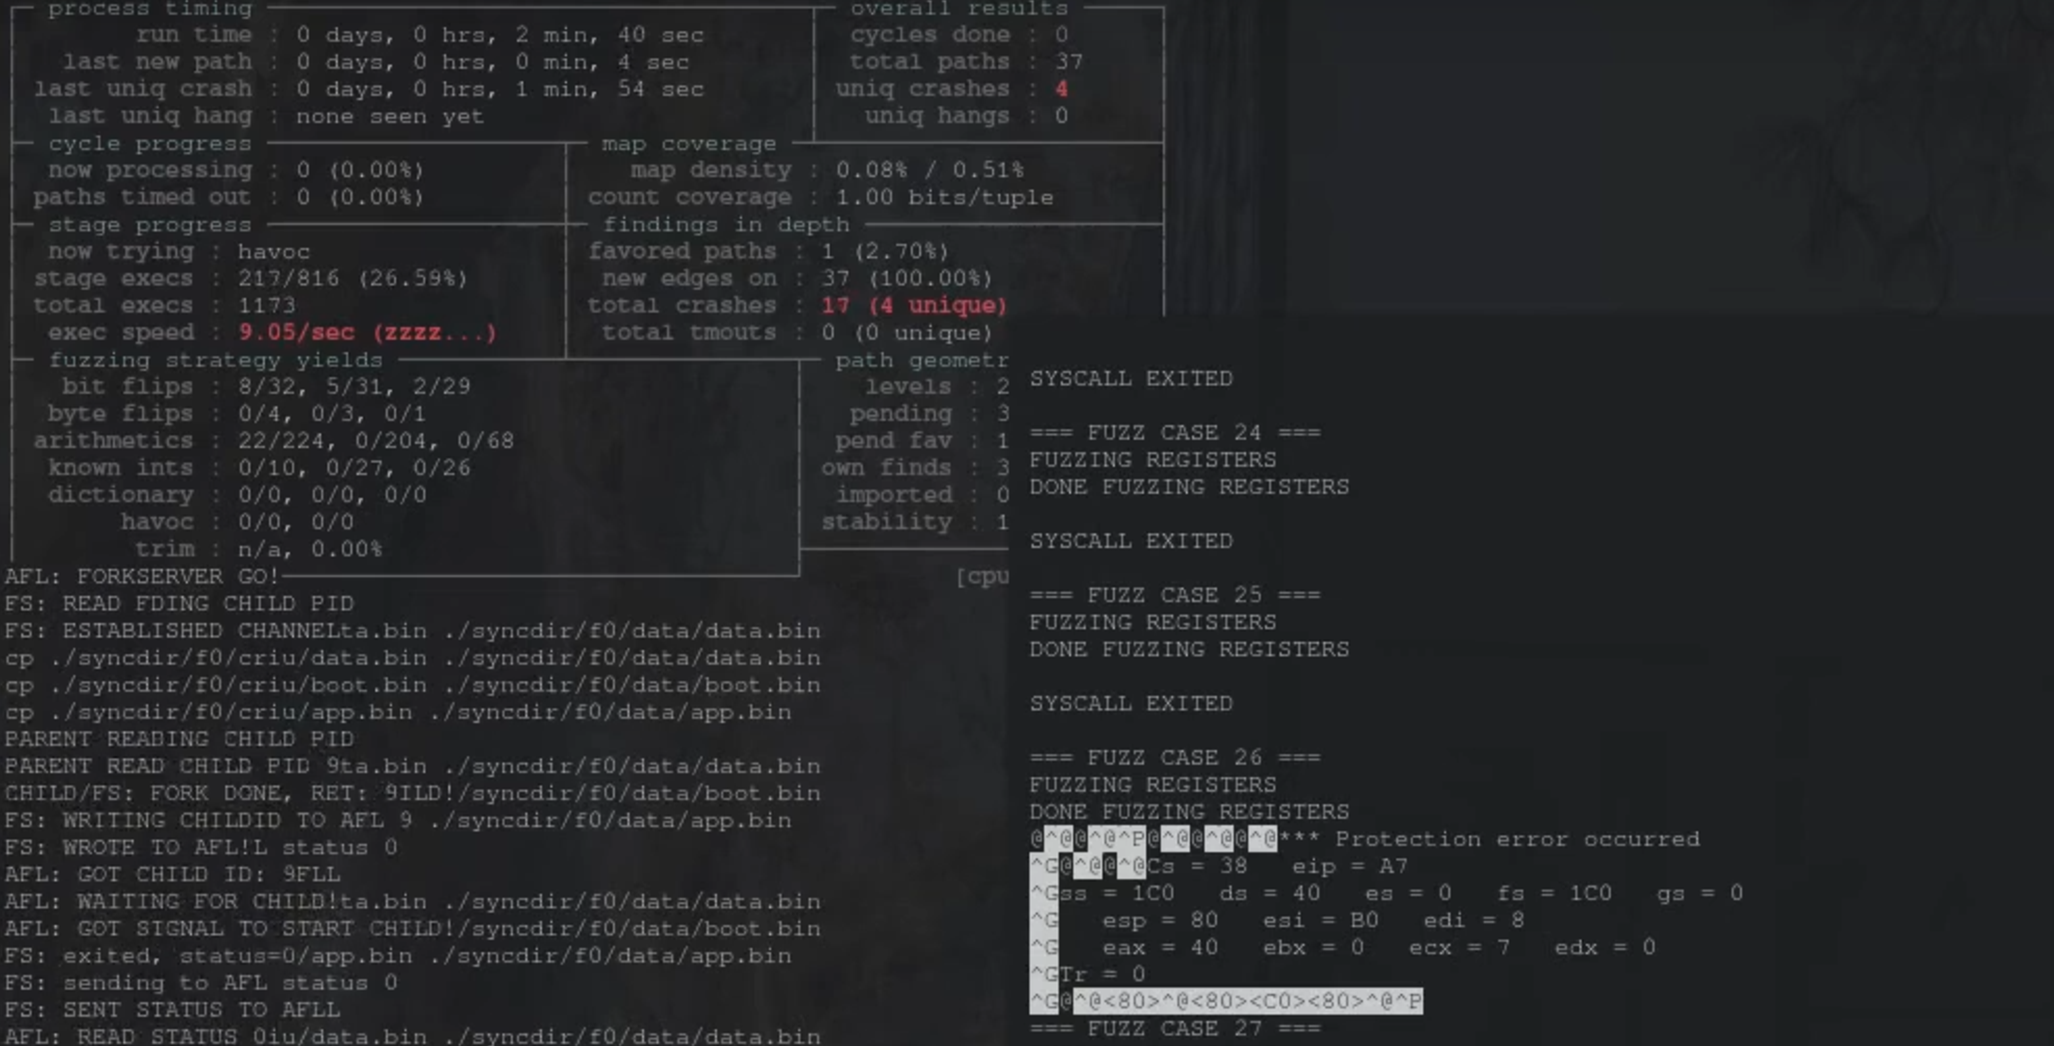
\includegraphics[width=\linewidth]{fuzzing-output}
\caption{A screenshot of the Jetset fuzzing framework (left) discovering a crash (right) in the CMU-900.}
\label{fig:fuzzing-out}
\end{figure}

\paragraph{CMU-900 Fuzzing}
The mainline QEMU distribution implements four of the peripheral devices used by the CMU-900 (the real-time clock, interrupt controller, interval timer, and serial controller).
We created a manual, ground-truth QEMU configuration mapping these devices at addresses expected by the code, which allowed us to compare the behavior of the emulated system with our synthetic devices against a QEMU configured with their full implementation.
As with the Raspberry Pi 2, we compared the behavior of the two systems by issuing system calls from unprivileged task 1.
A screenshot of the fuzzing framework is shown in Figure~\ref{fig:fuzzing-out}.

AFL found \cmuNumPathsDiscovered\ unique crash code paths during \cmuHoursFuzzed\ hours of fuzzing.
To compare the behavior of our two QEMU implementations (synthetic and manual), we compared the debugging console output produced by the \cmutarg.\footnote{
We would prefer to compare the synthetic device QEMU instance to the actual hardware, however, did not want to risk making the device inoperable, one explicit benefit of the emulated copies.
}
In the case of a successful system call return, the \cmutarg\ continues with its normal unprivileged task startup sequence.
In the event of a protection violation, the \cmutarg\ prints a wealth of debugging information, which we use to determine whether the two configurations behaved similarly.

Of the \cmuNumPathsDiscovered\ execution paths discovered by fuzzing, \cmuExactOutputMatches\ (\cmuPercentExactOutputToPaths) \ code paths exhibited identical behavior.
Another \cmuNearExactOutputMatches\ (\cmuPercentNearOutputToPaths) had the same outcome, but differed in the values in some of the registers.
The remaining \cmuNonExactOutputMatches\ (\cmuPercentNonExactOutputToPaths) also had the same outcome, but differed more extensively in the output generated.

Manual analysis of the \cmuNumPathsDiscovered\ execution paths led to
the discovery of a privilege escalation vulnerability.  The
vulnerability occurs because a single byte can be ``leaked'' from
unprivileged code into the offset of a call instruction in the VRTX
kernel.  One of the 256 potential values for this byte results in the
call targeting the middle of a function.  From here, a Return-Oriented
Program (ROP) chain can be used to modify the global descriptor table
(GDT).  A few instructions later, the GDT modification causes the
kernel protection error handler to fire.  However, the GDT
modification changes the base address of the data and stack segment
used by the handler so they overlap with an unprivileged data segment.
The handler includes a far call whose address is dependent upon a read
from the corrupted data segment.  A malicious address can be given to
this far call, leading to a second ROP chain which further modifies
the GDT.  This ROP chain changes the address range limits for
privileged code and transfers control to unprivileged, writable memory
while remaining in processor ring 0.

We were able to validate the exploit on another CMU-900 (one with a slightly different part number and
memory layout) after some minimal adaption and a live binary rewriting process paired with a local code execution exploit which ``poisoned'' the VRTX operating system with shim code. 
Due to small changes in the VRTX kernel between device versions, we discovered
the exploit's control transfer required supplying one ROP gadget address via a
segment rather than a data register and changing some gadget offsets.

\subsection{Leveraging Emulation in Avionics Exploit Development}
\label{sec:jetset-attack}
\label{sec:cmu-attack}

While the loading capability used to introduce software into the physical CMU was provided by the Triton Avionics Testbed~\cite{crow2019triton}, significant additional live binary instrumentation was needed to evaluate the exploit discovered above, and the techniques that were developed in this process allowed us to develop a mechanism for poisoning the CMU-900's VRTX operating system and led us to the discovery of three sets of messages capable of remotely disabling the CMU-900.
Because Aircraft Communication and Reporting System messages also have a ``broadcast'' mode, these messages could be used to crash a large number of CMU-900 devices simultaneously.
Due to their sensitivity, we omit the details of these messages from this dissertation and focus on techniques for their discovery, noting only that one message generates a buffer underflow where memory is allocated beyond the appropriate length and the other two cause excessive memory allocations which drain the availability of new heap memory.

The ability to run the CMU-900's VRTX operating system in an emulated environment was critical to the development and testing of these techniques and associated exploits.
The emulated copies of the CMU-900 allowed us to attempt numerous instrumentation approaches and gain visibility into implementation flaws, a task which would have been significantly more difficult on the physical device.

\paragraph{Bootloader and OS Initialization Replication}
Once our malicious software is loaded into the CMU-900 using the dataloader, control is effectively transferred entirely to the malicious code as a bootloader, negating any prior operating system and hardware device initialization.
It was thus necessary to replicate the bootloader and operating system initialization process in the emulator to ensure that the malicious code would be able to run in the same environment as it would on the physical device.
So, in this initial case, the malicious code would first relocate itself to an unused portion of RAM, transfer control to this new location, replicate the bootloader and initialization behavior necessary to reset the system back to an appropriate initial state, and then return control to to the original VRTX operating system.

Developing this replicated functionality required significant manual extraction and analysis of code using Ghidra.
The complexity of dealing with self-relocating code and the specific magic numbers involved for resource initialization led this ``poisoned'' version of the VRTX boot sequence required hundreds of lines of hand-written x86 assembly.
The development of this \emph{in situ} emulation also required significant universal quantification over possible relocation addresses as an alternative to the manual process of identifying a suitable relocation address, a unique benefit of using an emulated system, and served as one inspiration from the redaction attacks presented in Chapter~\ref{chap:info}.

\paragraph{Flash Code Relocation and Shim Injection}
For the purposes of analyzing the system for crashing inputs and testing the system call paths discovered by fuzzing in the previous section, it was not enough to \emph{replicate} the boot process.
Thus, we also performed binary rewriting of operating system code in order to inject instrumentation routines for the purposes of dynamic analysis.

This was complicated by the fact the CMU-900 executed a significant portion of its code out of flash memory, which was considered to be read-only in order to avoid damaging the physical unit.
It was therefore necessary to relocate the portions of code that were to be instrumented into unused, writable RAM memory, and update associated pointers.
This was a two stage process, first consisting of corrupting the interrupt vector table in order analyze portions of the code that were in use at runtime for critical functions and relevant to exploitation, and second, updating non-relative memory addressing data to point to the relocated code segments.

\begin{figure}
\begin{lstlisting}[language=C]
/* eax stores the original offset in the code. we read from this offset to get the relative offset the call lands at. We then change that offset so it is relative to the location of the trampoline call instruction. We then set it into the trampoline call instruction. */
"mov    $" TRAMPOLINE_LOC ",%ebx\n"
"add    $3,%eax\n"
"mov    %eax,1(%ebx)\n"
"sub    $3,%eax\n"
"mov    %eax,%ebx\n"
"add    $0x" RELOCATE_ACARS_CODE_BASE "00120,%eax\n"
"mov    (%eax),%eax\n"
"shl    $0x8,%eax\n"
"sar    $0x8,%eax\n"
/* Add three bytes to account for the three storage bytes */
"add    $0x3,%ebx\n"
/* Add relative base of call so it is relative to seg base */
"add    %ebx,%eax\n"
"sub    $" TRAMPOLINE_LOC_OFF ",%eax\n"
/* Subtract 10 bytes relative to the tramp call return  */
"sub    $0xA,%eax\n"
/* Write the jmp instruction of the trampoline loc */
"mov    $" TRAMPOLINE_LOC ",%ebx\n"
"mov    %eax,6(%ebx)\n"
\end{lstlisting}
\caption{Code for live binary rewriting of call instruction in the CMU-900 firmware.}
\label{fig:dynanal-code-cmu}
\end{figure}

However, once the appropriate relocation operations were complete, it was possible to inject additional shim code at arbitrary locations in system memory using binary rewriting tactics.
The primary rewriting tactic used was the augmentation of x86 call locations.
The precise method used is detailed in Section~\ref{sec:dynanal} of this dissertation, and code is given in Figure~\ref{fig:dynanal-code-cmu}
With shim instrumentation in place, it was trivial to manually identify potentially crashing inputs by examining data flows within the system.

\section{Open Challenges in Rehosting} 
\label{sec:jetset-limitations}

Returning to the primary subject of Jetset, the approach of targeted rehosting works well for firmware running on a variety of embedded system architectures across multiple application domains. 
However, this approach to peripheral modeling and system emulation is not without limitations, which we break down into \emph{internal} and \emph{external} semantic challenges.

\paragraph{Internal Semantics}
The paths explored by Jetset through firmware are not necessarily ones that may ever be returned by the hardware in the original system; however, the path taken is one that is acceptable to the firmware\textemdash no interaction with any of the peripherals results in a boot failure.
While the execution of firmware running on physical hardware is constrained in its behavior by how the physical peripherals really behave, these system constraints are external to the firmware and cannot be inferred without auxiliary information about its behavior.
To effectively emulate a system, it is not necessary not only to explore a single execution path, but to reveal the connections and meaning implied by multiple execution paths, a topic we will approach in Chapter~\ref{chap:info} and refine in Chapter~\ref{chap:integreat}.

\paragraph{External Semantics}
Jetset does \textit{targeted rehosting} in that it only constructs an emulator that is sufficient to emulate the software component-under-test.
However, rehosting may have no method of deducing the semantics of devices that the system depends upon if the only information it considers is that which is contained within the system specification which remains after these devices are removed, e.g. firmware.
Jetset could be extended to synthesize more complex, stateful peripheral models as well as identify known peripherals with existing emulator implementations using additional information from external sources.

Included in external semantics is the information requires to solve the dynamic analysis challenges presented by Section~\ref{sec:jetset-attack}, which exist outside of the simple execution of a given system model.
While this information is of less general application, it still plays a critical role in quantifying the security of the emulated system, as evidenced by its utility in exploit development.

\section{Summary}

In this chapter, we discussed one approach to the emulation of complex systems, targeted firmware rehosting.
The benefit of this approach is its ability to synthesize peripheral hardware devices for the analysis of real-world embedded systems.
Particularly, it considers the available information about the system to derive models of unknown components.
In the next chapter, we will develop an alternative approach which addresses some of the shortcomings of looking at a strict derivation from available information for resolving unknown components: universal quantification over possible missing information, and see how this approach applies to the security of real-world redactions.
